\section{Experiments}\label{sec:experiments}

In this section we describe the results of experiments comparing
the run time of \Sparrow\ with those of two leading implementations of
boosted trees: XGBoost and LightGBM.


\begin{table}[]
\centering
\label{table-exp}
\begin{tabular}{|l|l|c|c|}
\hline
Memory       & \Sparrow         & XGBoost             & LightGBM       \\ \hline
16 GB        & 18.5             & 3224.7 (on disk) & (crash)        \\
32 GB        & 17.9             & 1705.8 (on disk) & (crash)        \\
72 GB        & 21.9             & 1497.7 (on disk) & 108.1          \\
144 GB       & 19.6             & 241.4 (in memory)   & 109.4          \\ \hline

% \end{tabular}
% \vspace{0.2cm}
% \begin{tabular}{|l|l|c|c|}
%                 & \Sparrow         & XGBoost             & LightGBM       \\ \hline
\#~Rules  & 189    & 400                 & 400            \\ \hline
\end{tabular}

\vspace{0.2cm}

\caption{Comparison of the total training time on
the splice site detection task (minutes) and the number
of rules in the final ensemble when it converges}
\end{table}


\subsection{Setup}

We use a large dataset that was used in other studies of large scale
learning on detecting human acceptor splice site~\cite{sonnenburg_coffin_2010, agarwal_reliable_2014}.
The learning task is binary classification.
We use the same training dataset of 50\,M samples as in the other work,
and validate the model on the testing data set of 4.6\,M samples.
The training dataset on disk takes over 27\,GB in size.

In current implementation of \Sparrow, we restrict our trees to one
level so-called ``decision stumps''. We plan to perform comparisons
using multi-level trees and more than two labels. We expect similar
runtime performance there. To generate comparable models,
we also train decision stumps in XGBoost and LightGBM
(by setting the maximum tree depth to 1).

Both XGBoost and LightGBM are highly optimized, and support multiple
tree construction algorithms.
For XGBoost, we chose approximate greedy algorithm which is its fastest method.
LightGBM supports using sampling in the training,
which they called \textit{Gradient-based One-Side Sampling} (GOSS).
GOSS keeps a fixed percentage of examples with large gradients,
and then randomly sample from remaining examples with small gradients.
We selected GOSS as the tree construction algorithm for LightGBM.

All algorithms in comparison optimize the exponential loss as defined in AdaBoost.
We also evaluated the final model by calculating its area under precision-recall
curve (AUPRC) on the testing dataset.

Finally, the experiments are all conducted on EC2 instances from Amazon Web Services.
We ran the evaluations on four different instance types with increasing memory capacities,
specifically
16\,GB (\texttt{c5d.2xlarge}), 32\,GB (\texttt{c5d.2xlarge}),
72\,GB (\texttt{c5d.9xlarge}), and 144\,GB (\texttt{c5d.18xlarge}).
The training time in each configuration is listed in Table~\ref{table-exp}.

\begin{table}[]
\centering
\label{table-per-tree}
\begin{tabular}{|l|l|c|c|}
\hline
Memory       & \Sparrow         & XGBoost             & LightGBM       \\ \hline
16 GB        & 5.7             & 483.7 (on disk) & (crash)        \\
32 GB        & 5.6             & 255.9 (on disk) & (crash)        \\
72 GB        & 6.8             & 224.7 (on disk) & 16.2          \\
144 GB       & 6.6             & 36.2 (in memory)   & 16.4          \\ \hline
\end{tabular}

\vspace{0.2cm}

\caption{Comparison of the per-tree training time
on the splice site detection task (seconds)}
\end{table}


\subsection{Evaluation}

Performance of each of the algorithm in terms of
the exponential loss as a function of time on the testing dataset is given in
Figure~\ref{fig:loss}. Observe that all algorithms achieve similar
final loss, but it takes them different amount of time to reach that
final loss. We summarize these differences in Table~\ref{table-exp} by
using the convergence time to an almost optimal loss of
$0.061$. Observe  XGBoost off-memory is about 27
times slower than a single \Sparrow\ worker which is also off-memory. That
time improves by another factor of 3.2 by using 10 machines instead of 1.

In Figure~\ref{fig:auprc} we perform the comparison in terms of
AUPRC. The results are similar in terms of speed. However, in this
case XGBoost and LightGBM ultimately achieve a slightly better
AUPRC. This is baffling, because all algorithms work by minimizing
exponential loss.

\begin{figure}[t]
    \centering
    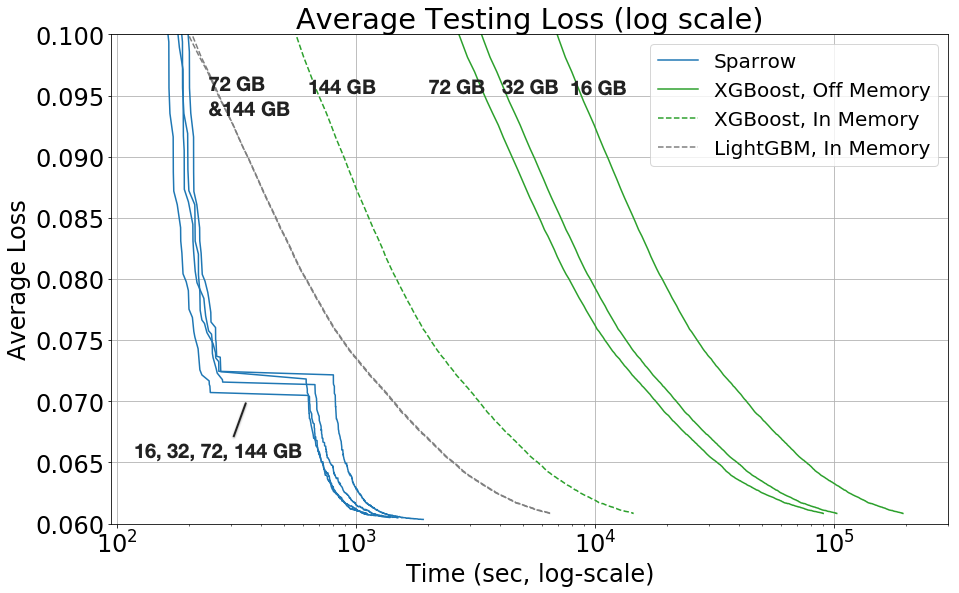
\includegraphics[width=0.5\textwidth]{figs/splice-loss2m.png}
    \caption{Comparing the average loss on the testing data using \Sparrow, XGBoost, and LightGBM, lower is better.
        The period of time that the loss is constant for \Sparrow\ is when the algorithm is generating a new sample set.}~\label{fig:loss}
\end{figure}



\begin{figure}[t]
    \centering
    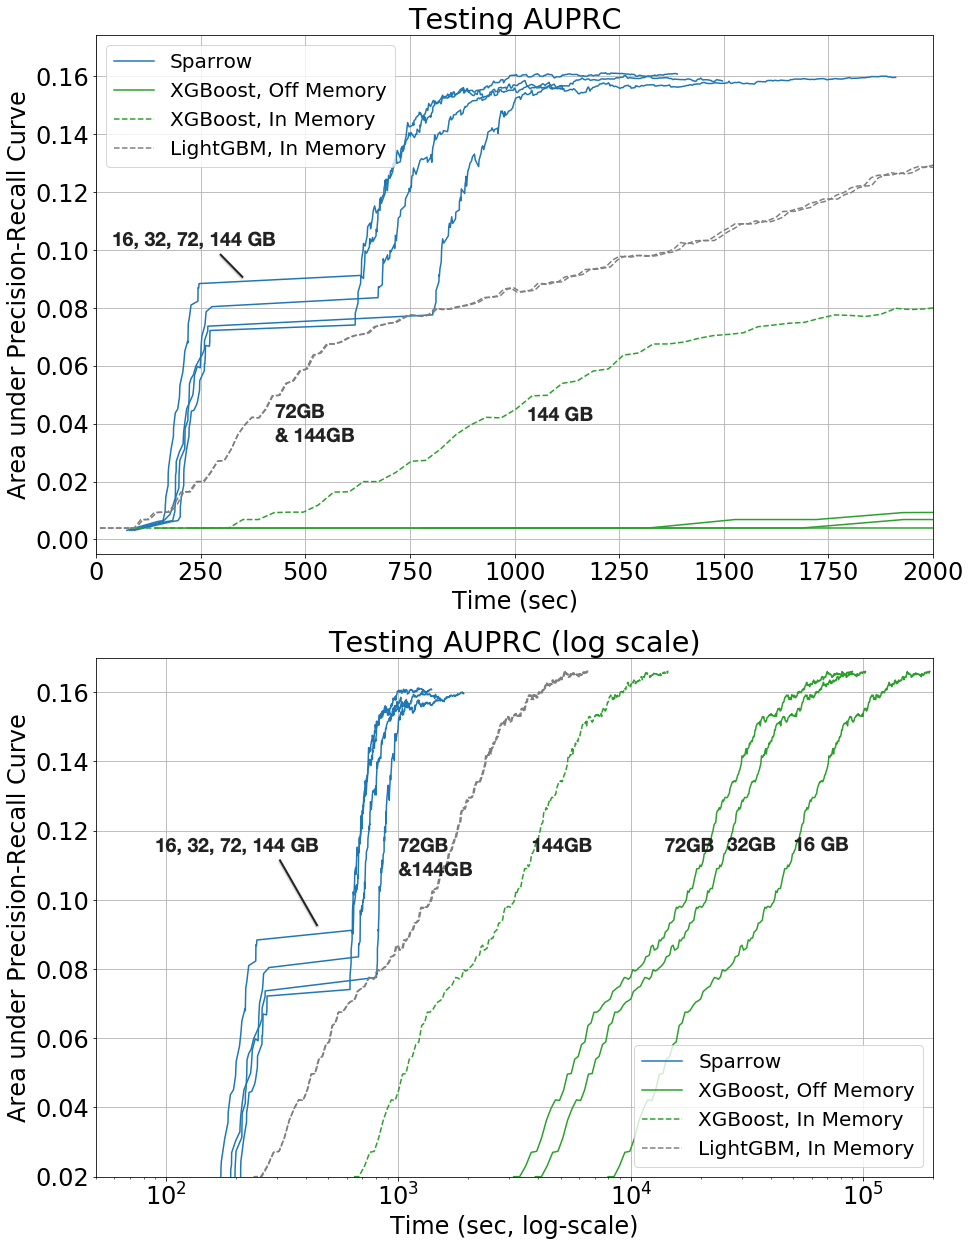
\includegraphics[width=0.5\textwidth]{figs/splice-auprc2m.png}
    \caption{Comparing the area under the precision-recall curve (AUPRC) on the testing data
    using \Sparrow, XGBoost, and LightGBM, higher is better.
    (left) Normal scale, clipped on right.
    (right) Log scale, clipped on left.
    The period of time that the AUPRC is constant for \Sparrow\ is when the algorithm is generating a new sample set.}~\label{fig:auprc}
\end{figure}


\section{Future Work}\label{sec:Conclusion}
Our preliminary results show that early stopping and selective
sampling can dramatically speed up boosting algorithms on large
real-world datasets.

The source code for sparrow is available for {\tt }

We have several directions for future work.

First, \Sparrow\ is currently limited boosting stumps and to binary
classification. We plan to extend \Sparrow\ to deep trees and to allow
more than two labels. We will then run it on many more data sets.

Second, our work shows that sampling from memory can take an
inordinate amount of time when the training set is large and the
weights are highly skewed. We have developed a stratified sampling
algrithm that significantly reduces this problem.

Third, we are working on a parallelized version of \Sparrow\ which
uses a  novel type of asynchronous communication protocol.

Fourth, our current implementation of \Sparrow\ does not take
advantage of multi-core machines as much as LightGBM does. We plan to
address that problem.




